\documentclass[]{tufte-handout}

% ams
\usepackage{amssymb,amsmath}

\usepackage{ifxetex,ifluatex}
\usepackage{fixltx2e} % provides \textsubscript
\ifnum 0\ifxetex 1\fi\ifluatex 1\fi=0 % if pdftex
  \usepackage[T1]{fontenc}
  \usepackage[utf8]{inputenc}
\else % if luatex or xelatex
  \makeatletter
  \@ifpackageloaded{fontspec}{}{\usepackage{fontspec}}
  \makeatother
  \defaultfontfeatures{Ligatures=TeX,Scale=MatchLowercase}
  \makeatletter
  \@ifpackageloaded{soul}{
     \renewcommand\allcapsspacing[1]{{\addfontfeature{LetterSpace=15}#1}}
     \renewcommand\smallcapsspacing[1]{{\addfontfeature{LetterSpace=10}#1}}
   }{}
  \makeatother

\fi

% graphix
\usepackage{graphicx}
\setkeys{Gin}{width=\linewidth,totalheight=\textheight,keepaspectratio}

% booktabs
\usepackage{booktabs}

% url
\usepackage{url}

% hyperref
\usepackage{hyperref}

% units.
\usepackage{units}


\setcounter{secnumdepth}{-1}

% citations
\usepackage{natbib}
\bibliographystyle{plainnat}


% pandoc syntax highlighting
\usepackage{color}
\usepackage{fancyvrb}
\newcommand{\VerbBar}{|}
\newcommand{\VERB}{\Verb[commandchars=\\\{\}]}
\DefineVerbatimEnvironment{Highlighting}{Verbatim}{commandchars=\\\{\}}
% Add ',fontsize=\small' for more characters per line
\newenvironment{Shaded}{}{}
\newcommand{\AlertTok}[1]{\textcolor[rgb]{1.00,0.00,0.00}{\textbf{#1}}}
\newcommand{\AnnotationTok}[1]{\textcolor[rgb]{0.38,0.63,0.69}{\textbf{\textit{#1}}}}
\newcommand{\AttributeTok}[1]{\textcolor[rgb]{0.49,0.56,0.16}{#1}}
\newcommand{\BaseNTok}[1]{\textcolor[rgb]{0.25,0.63,0.44}{#1}}
\newcommand{\BuiltInTok}[1]{#1}
\newcommand{\CharTok}[1]{\textcolor[rgb]{0.25,0.44,0.63}{#1}}
\newcommand{\CommentTok}[1]{\textcolor[rgb]{0.38,0.63,0.69}{\textit{#1}}}
\newcommand{\CommentVarTok}[1]{\textcolor[rgb]{0.38,0.63,0.69}{\textbf{\textit{#1}}}}
\newcommand{\ConstantTok}[1]{\textcolor[rgb]{0.53,0.00,0.00}{#1}}
\newcommand{\ControlFlowTok}[1]{\textcolor[rgb]{0.00,0.44,0.13}{\textbf{#1}}}
\newcommand{\DataTypeTok}[1]{\textcolor[rgb]{0.56,0.13,0.00}{#1}}
\newcommand{\DecValTok}[1]{\textcolor[rgb]{0.25,0.63,0.44}{#1}}
\newcommand{\DocumentationTok}[1]{\textcolor[rgb]{0.73,0.13,0.13}{\textit{#1}}}
\newcommand{\ErrorTok}[1]{\textcolor[rgb]{1.00,0.00,0.00}{\textbf{#1}}}
\newcommand{\ExtensionTok}[1]{#1}
\newcommand{\FloatTok}[1]{\textcolor[rgb]{0.25,0.63,0.44}{#1}}
\newcommand{\FunctionTok}[1]{\textcolor[rgb]{0.02,0.16,0.49}{#1}}
\newcommand{\ImportTok}[1]{#1}
\newcommand{\InformationTok}[1]{\textcolor[rgb]{0.38,0.63,0.69}{\textbf{\textit{#1}}}}
\newcommand{\KeywordTok}[1]{\textcolor[rgb]{0.00,0.44,0.13}{\textbf{#1}}}
\newcommand{\NormalTok}[1]{#1}
\newcommand{\OperatorTok}[1]{\textcolor[rgb]{0.40,0.40,0.40}{#1}}
\newcommand{\OtherTok}[1]{\textcolor[rgb]{0.00,0.44,0.13}{#1}}
\newcommand{\PreprocessorTok}[1]{\textcolor[rgb]{0.74,0.48,0.00}{#1}}
\newcommand{\RegionMarkerTok}[1]{#1}
\newcommand{\SpecialCharTok}[1]{\textcolor[rgb]{0.25,0.44,0.63}{#1}}
\newcommand{\SpecialStringTok}[1]{\textcolor[rgb]{0.73,0.40,0.53}{#1}}
\newcommand{\StringTok}[1]{\textcolor[rgb]{0.25,0.44,0.63}{#1}}
\newcommand{\VariableTok}[1]{\textcolor[rgb]{0.10,0.09,0.49}{#1}}
\newcommand{\VerbatimStringTok}[1]{\textcolor[rgb]{0.25,0.44,0.63}{#1}}
\newcommand{\WarningTok}[1]{\textcolor[rgb]{0.38,0.63,0.69}{\textbf{\textit{#1}}}}

% longtable
\usepackage{longtable,booktabs}

% multiplecol
\usepackage{multicol}

% strikeout
\usepackage[normalem]{ulem}

% morefloats
\usepackage{morefloats}


% tightlist macro required by pandoc >= 1.14
\providecommand{\tightlist}{%
  \setlength{\itemsep}{0pt}\setlength{\parskip}{0pt}}

% title / author / date
\title[分散の加法性を視覚的に理解する]{分散の加法性を視覚的に理解する}
\author{Sampo Suzuki, CC 4.0 BY-NC-SA}
\date{2021-05-31}

% --- 参考資料 ----------------------------------------------------------------
% https://github.com/Gedevan-Aleksizde/Japan.R2019/blob/master/latex/preamble.tex
% https://teastat.blogspot.com/2019/01/bookdown.html

% --- Packages ----------------------------------------------------------------
% 日本語とtufte, kableExtraを使うために必要なTeXパッケージ指定
% tufteではA4サイズの指定が不可能
%  A4 210mm x 297mm
%   \usepackage[a4paper, total={6.5in, 9.5in}]{geometry}
%   \usepackage{indentfirst}   # tinytexのリポジトリには存在しない?
% \usepackage[a4paper, total={160mm, 247mm}, left=25mm, top=25mm]{geometry}
% \usepackage[pdfbox,tombo]{gentombow}  % トンボを設定する場合は有効にする
% \usepackage{ifthen}                     % 条件分岐用 \ifthenelse{条件}{T}{F}
\usepackage{booktabs}                   % ここからkableExtra用パッケージ
\usepackage{longtable}                  % 
\usepackage{array}                      % 
\usepackage{multirow}                   % 
\usepackage{wrapfig}                    % 
\usepackage{float}                      % 
\usepackage{colortbl}                   % 
\usepackage{pdflscape}                  % 
\usepackage{tabu}                       % 
\usepackage{threeparttable}             % 
\usepackage{threeparttablex}            % 
\usepackage[normalem]{ulem}             % 
\usepackage{inputenc}                   % 
\usepackage{makecell}                   % 
\usepackage{xcolor}                     % ここまでkableExtra用
\usepackage{amsmath}                    % 
\usepackage{fontawesome5}               % fontawesomeを使うために必要
\usepackage{subfig}
\usepackage{xeCJK}                      % 以下、日本語フォント用に必要
\usepackage[noto]{zxjafont}             % Linux環境ではこちを指定
% \usepackage[haranoaji]{zxjafont}      % Windows環境ではこちらを指定する
\usepackage{zxjatype}
\usepackage{pxrubrica}                  % ルビ用
\usepackage{hyperref}                   % ハイパーリンク用必要?

% --- Index ------------------------------------------------------------------
% https://texwiki.texjp.org/?%E7%B4%A2%E5%BC%95%E4%BD%9C%E6%88%90
% これを指定するとIndex(索引)は作成されるが参照ページがズレる
% 中間ファイルの.indではページはズレていないので、その後の結合処理がおかしい
% \usepackage{makeidx}
% \makeindex
% \usepackage{showidx}                  % 索引確認用

% --- Table of Contentes ------------------------------------------------------
% TOCにLOT(List of Tables), LOF(List of Figures), Bibliography, Indexを表示
% \usepackage[nottoc]{tocbibind}

% --- Fonts -------------------------------------------------------------------
% フォントしては index.html でも可能(pandoc用オプションは index.htmlにて)
% \setCJKmonofont{Source Han Code JP}
\setmonofont{Source Han Code JP}
% \setjamonofont{Source Han Code JP}

% ## 日本語フォントの扱いについてはzxjafontパッケージの解説を参照のこと
% # https://mirror.las.iastate.edu/tex-archive/language/japanese/zxjafont/zxjafont.pdf
% #
% ## Windows環境ではなぜかNotoフォントが認識されないので源ノシリーズベースの
% ## 原ノ味フォントかIPAexフォントを利用する(原ノ味はtlmgrでインストール可)
% # \usepackage[haranoaji]{zxjafont}
% # \usepackage[ipaex]{zxjafont}
% #
% ## Windows環境でNotoフォントを指定したい場合は以下のようにheader-includeで
% ## 個別に指定する(setCJKxxxfotnの指定は必要?)
% # \setmainfont{NotoSerifCJKjp-Regular.otf}[BoldFont=NotoSerifCJKjp-Bold.otf]
% # \setsansfont{NotoSansCJKjp-Regular.otf}[BoldFont=NotoSansCJKjp-Bold.otf]
% # \setmonofont{NotoSansMonoCJKjp-Regular.otf}[BoldFont=NotoSansMonoCJKjp-Bold.otf]
% ## モノフォントは源ノ角コード(Source Code Proの日本語版)がおすゝめ
% # \setmonofont{SourceHanCodeJP-Regular.otf}[BoldFont=SourceHanCodeJPS-Bold.otf]

\begin{document}

\maketitle




\hypertarget{introduction}{%
\section{\texorpdfstring{\textbf{Introduction}}{Introduction}}\label{introduction}}

 2021年度データ分析勉強会のテキストである『統計解析のはなし』\citep{ToukeiKaisekinoHanashi}の「標本が2つになれば」(P26〜)には分散の加法性の話が出てきます。分散の加法性は理解できるようでいて、理解できていないので、\textbf{R}を使って分散の加法性を可視化しながら説明してみます。

以降、平均値\(\mu\)、標準偏差\(\sigma\)、分散\(\sigma^2\)である正規分布を\(N(\mu, \sigma^2)\)と表記します。

 

\hypertarget{ux52a0ux6cd5ux6027ux3092ux53efux8996ux5316ux3059ux308b}{%
\section{\texorpdfstring{\textbf{加法性を可視化する}}{加法性を可視化する}}\label{ux52a0ux6cd5ux6027ux3092ux53efux8996ux5316ux3059ux308b}}

 以下の平均値と標準偏差を持つ二つの正規分布を\texttt{rnorm()}関数による正規分布乱数を用いて作成\footnote{n
  = \ensuremath{5\times 10^{6}}個の値を作成しています}します。

\begin{longtable}[]{@{}lccl@{}}
\caption{二つの正規分布}\tabularnewline
\toprule
正規分布 & 平均 & 標準偏差 & 備考 \\
\midrule
\endfirsthead
\toprule
正規分布 & 平均 & 標準偏差 & 備考 \\
\midrule
\endhead
\(N(\mu_a, \sigma^2_a)\) & \(\mu_a = 10\) & \(\sigma_a = 10\) & \\
\(N(\mu_b, \sigma^2_b)\) & \(\mu_b = 30\) & \(\sigma_b = 10\) & \\
\bottomrule
\end{longtable}

\begin{Shaded}
\begin{Highlighting}[numbers=left,,]
\NormalTok{a }\OtherTok{\textless{}{-}} \FunctionTok{rnorm}\NormalTok{(n, }\AttributeTok{mean =} \DecValTok{10}\NormalTok{, }\AttributeTok{sd =} \DecValTok{10}\NormalTok{)}
\NormalTok{b }\OtherTok{\textless{}{-}} \FunctionTok{rnorm}\NormalTok{(n, }\AttributeTok{mean =} \DecValTok{30}\NormalTok{, }\AttributeTok{sd =} \DecValTok{10}\NormalTok{)}
\end{Highlighting}
\end{Shaded}

\begin{marginfigure}

{\centering 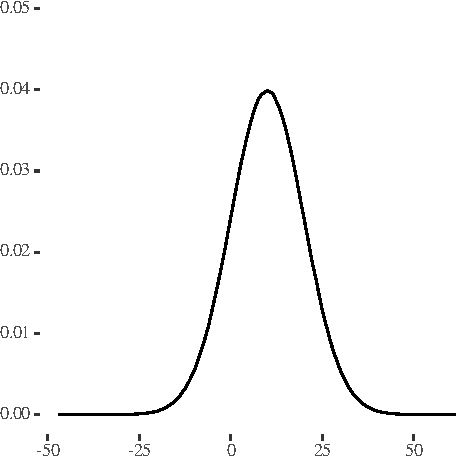
\includegraphics{AdditivityOfVariance_files/figure-latex/unnamed-chunk-2-1} 

}

\caption[$N(\mu_a, \sigma^2_a)$の分布]{$N(\mu_a, \sigma^2_a)$の分布}\label{fig:unnamed-chunk-2}
\end{marginfigure}

\begin{marginfigure}

{\centering 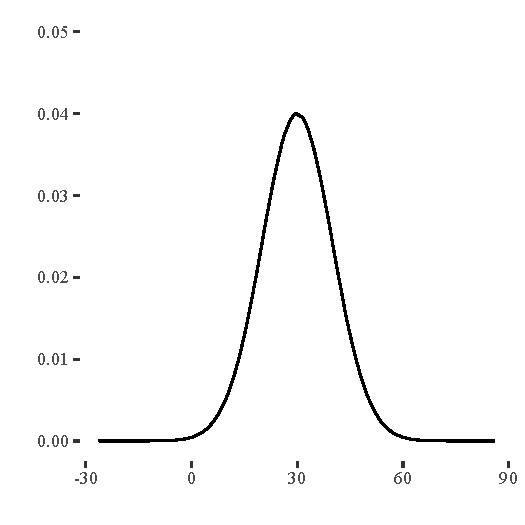
\includegraphics{AdditivityOfVariance_files/figure-latex/unnamed-chunk-3-1} 

}

\caption[$N(\mu_b, \sigma^2_bb)$の分布]{$N(\mu_b, \sigma^2_bb)$の分布}\label{fig:unnamed-chunk-3}
\end{marginfigure}

\begin{longtable}[]{@{}lcccl@{}}
\caption{二つの正規分布の要約統計量}\tabularnewline
\toprule
正規分布 & 平均 & 分散 & 標準偏差 & 備考 \\
\midrule
\endfirsthead
\toprule
正規分布 & 平均 & 分散 & 標準偏差 & 備考 \\
\midrule
\endhead
\(N(\mu_a, \sigma^2_a)\) & 10.0016756 & 99.9836706 & 9.9991835 & \\
\(N(\mu_b, \sigma^2_b)\) & 29.9992382 & 99.9499051 & 9.9974949 & \\
\bottomrule
\end{longtable}

この二つの正規分布\(N(\mu_a, \sigma^2_a)\)と\(N(\mu_b,\sigma^2_b)\)からランダムサンプリングにより一つずづ値を取り出して加算します。すなわち
 
\[N(\mu_a, \sigma^2_a)\mbox{ から取り出した値} + N(\mu_b,\sigma^2_b)\mbox{ から取り出した値}\]

という新しい値を作成します。取り出した値は元に戻し、同様の取り出し、加算を繰り返すと以下のようなデータが作成できます。ここではスペースの都合で先頭から限定して表示しています。

\begin{Shaded}
\begin{Highlighting}[numbers=left,,]
\NormalTok{c }\OtherTok{\textless{}{-}} \FunctionTok{c}\NormalTok{(}\FunctionTok{sample}\NormalTok{(a, n, }\AttributeTok{replace =} \ConstantTok{TRUE}\NormalTok{) }\SpecialCharTok{+} \FunctionTok{sample}\NormalTok{(b, n, }\AttributeTok{replace =} \ConstantTok{TRUE}\NormalTok{))}
\FunctionTok{head}\NormalTok{(c, }\DecValTok{50}\NormalTok{)}
\end{Highlighting}
\end{Shaded}

\begin{verbatim}
##  [1] 46.1163151 20.3791277 53.3515673 21.8963015 61.1246494 51.2528823
##  [7] 31.6871108 39.2162349 17.5558542 20.7128908 59.3459501 14.2180864
## [13] -0.2665056 25.7861722 36.7150493 57.6574579 44.5347530 27.7907453
## [19] 41.6449701 45.0677697 29.9428047 27.7026317 20.0414525 47.8090035
## [25] 27.3501016 23.2370535 55.4529451 56.2804943 39.5785953 45.5288645
## [31] 40.5379614 25.2187384  7.5660458 28.6497265 32.3198940 54.7287173
## [37] 34.1525732 28.1064348 31.9661833 51.1781650 40.7792296 41.0413417
## [43] 60.3036364 34.8352682 51.7803487 12.9406436 37.7692407 43.7219224
## [49] 48.3308208 44.2242397
\end{verbatim}

分散の加法性により上記のデータは\(N(\mu_a + \mu_b, \sigma^2_a + \sigma^2_b))\)という正規分布になるはずですが実際はどうでしょう。各正規分布の平均値と分散を比較します。

\begin{longtable}[]{@{}lccl@{}}
\caption{各分布の要約統計量}\tabularnewline
\toprule
正規分布 & 平均 & 分散 & 備考 \\
\midrule
\endfirsthead
\toprule
正規分布 & 平均 & 分散 & 備考 \\
\midrule
\endhead
\(N(\mu_a, \sigma^2_a)\) & 10.0016756 & 99.9836706 & 元の分布 \\
\(N(\mu_b, \sigma^2_b)\) & 29.9992382 & 99.9499051 & 元の分布 \\
\(N(\mu_a + \mu_b, \sigma^2_a + \sigma^2_b))\) & 40.0009138 &
199.9335756 & 分散の加法性 \\
\(N(\mu_c, \sigma^2_c)\) & 39.9967145 & 200.0743299 & 実際の分布 \\
\bottomrule
\end{longtable}

このように確かに分散の加法性が成り立っており、正規分布\(N(\mu_a, \sigma^2_a)\)や\(N(\mu_b,\sigma^2_b)\)より横に広がった正規分布になっていることが分かります。

\begin{marginfigure}

{\centering 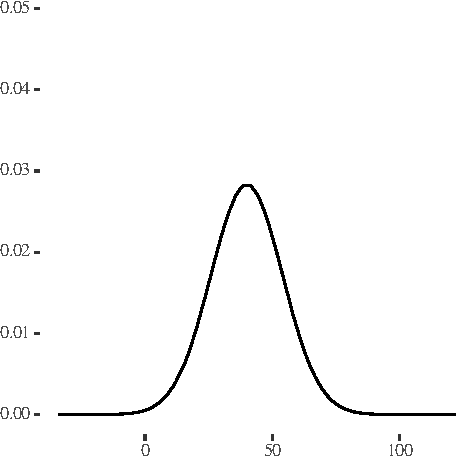
\includegraphics{AdditivityOfVariance_files/figure-latex/unnamed-chunk-5-1} 

}

\caption[$N(\mu_c, \sigma^2_c)$の分布]{$N(\mu_c, \sigma^2_c)$の分布}\label{fig:unnamed-chunk-5}
\end{marginfigure}

\newpage

\hypertarget{ux540cux4e00ux306eux6b63ux898fux5206ux5e03ux304bux3089ux53d6ux308aux51faux3057ux5024ux3092ux52a0ux7b97ux3057ux305fux5834ux5408}{%
\subsection{\texorpdfstring{\textbf{同一の正規分布から取り出し値を加算した場合}}{同一の正規分布から取り出し値を加算した場合}}\label{ux540cux4e00ux306eux6b63ux898fux5206ux5e03ux304bux3089ux53d6ux308aux51faux3057ux5024ux3092ux52a0ux7b97ux3057ux305fux5834ux5408}}

 次に二つの正規分布\(N(\mu_a, \sigma^2_a)\)と\(N(\mu_b,\sigma^2_b)\)がまったく等しいと仮定します。つまり

\[\mu_a = \mu_b = \mu_d\]

\[\sigma_a = \sigma_b = \sigma_d\]

という正規分布\(N(\mu_d, \sigma^2_d)\)を作成します。

\begin{Shaded}
\begin{Highlighting}[numbers=left,,]
\NormalTok{d }\OtherTok{\textless{}{-}} \FunctionTok{rnorm}\NormalTok{(n, }\AttributeTok{mean =} \DecValTok{10}\NormalTok{, }\AttributeTok{sd =} \DecValTok{10}\NormalTok{)}
\FunctionTok{head}\NormalTok{(d, }\DecValTok{50}\NormalTok{)}
\end{Highlighting}
\end{Shaded}

\begin{verbatim}
##  [1]  10.4718478   4.9849636  24.4768738   5.9558301   7.7480742  27.4413166
##  [7]  21.1164196   9.3571719  17.2357327  12.3316145  26.9292925   7.1489398
## [13]   3.7063110  23.2323883  -8.4626318   5.5915979  -9.7637977  21.3708252
## [19]   5.3004719  18.2108842  17.0170253  16.5061865  25.3001358  15.1217001
## [25]   4.4774172   6.0094778   8.5488500  13.9068968  34.5300485   2.7411102
## [31]   3.2848838   9.3957845  24.7347964   0.3809330   5.7002271  16.1209396
## [37]  14.4848248  24.6707233  -0.1087532  11.4830700   7.1821467   1.8100113
## [43]  13.7401719 -11.3177720  27.2871844  21.5304871  12.7569856  10.1043822
## [49]  28.2371418  18.4233884
\end{verbatim}

この正規分布\(N(\mu_d, \sigma^2_d)\)から先程と同様にランダムサンプリングにより一つずづ値を取り出して加算しますが、今回は同一正規分布\(N(\mu_d, \sigma^2_d)\)ですので、二つ取り出します。取り出した値は元の正規分布に戻し同様の操作を繰り返します。

 

\begin{Shaded}
\begin{Highlighting}[numbers=left,,]
\NormalTok{e }\OtherTok{\textless{}{-}} \FunctionTok{c}\NormalTok{(}\FunctionTok{sample}\NormalTok{(d, n, }\AttributeTok{replace =} \ConstantTok{TRUE}\NormalTok{) }\SpecialCharTok{+} \FunctionTok{sample}\NormalTok{(d, n, }\AttributeTok{replace =} \ConstantTok{TRUE}\NormalTok{))}
\FunctionTok{head}\NormalTok{(e, }\DecValTok{50}\NormalTok{)}
\end{Highlighting}
\end{Shaded}

\begin{verbatim}
##  [1]   8.994299  34.512526   8.023292   1.853060  11.134472  13.456867
##  [7]  -1.236911  43.042327   9.688241  26.203479  32.099955  10.895178
## [13]  28.656876  21.727965  25.561257  18.999813  17.953008  27.535234
## [19]  23.392168  24.511423  63.000654  20.293859  18.665178   3.437621
## [25]  37.886192   2.147762  22.421276  14.121936   8.985141  16.292188
## [31]  23.056984  28.247759  37.227212  21.648009  25.883282   5.507856
## [37]   4.249043  26.259230  26.205216  42.227126  30.747036  13.058043
## [43]  26.658647  28.697299   4.633673  25.371136 -16.056406  22.763227
## [49]  12.493839   8.654325
\end{verbatim}

\newpage

分散の加法性により以下が成り立ちます。

\[N(\mu_d + \mu_d, \sigma^2_d + \sigma^2_d) = N(2\mu_d, 2\sigma^2_d)\]

つまり、正規分布\(N(\mu_d, \sigma^2_d)\)から取り出した二つの値の和である正規分布\(N(\mu_e, \sigma^2_e)\)は

\begin{longtable}[]{@{}
  >{\raggedright\arraybackslash}p{(\columnwidth - 8\tabcolsep) * \real{0.16}}
  >{\centering\arraybackslash}p{(\columnwidth - 8\tabcolsep) * \real{0.20}}
  >{\centering\arraybackslash}p{(\columnwidth - 8\tabcolsep) * \real{0.20}}
  >{\centering\arraybackslash}p{(\columnwidth - 8\tabcolsep) * \real{0.36}}
  >{\raggedright\arraybackslash}p{(\columnwidth - 8\tabcolsep) * \real{0.09}}@{}}
\caption{加法性による要約統計量}\tabularnewline
\toprule
正規分布 & 平均 & 分散 & 標準偏差 & 備考 \\
\midrule
\endfirsthead
\toprule
正規分布 & 平均 & 分散 & 標準偏差 & 備考 \\
\midrule
\endhead
\(N(\mu_e, \sigma^2_e)\) & \(2 \mu_d\) & \(2 \sigma^2_d\) &
\(\sqrt{2 \sigma^2_d} = \sqrt{2}\sigma_d\) & \\
\bottomrule
\end{longtable}

という正規分布をすることになります。加法性と実際の正規分布を比べてみると

\begin{longtable}[]{@{}lccl@{}}
\caption{各分布の要約統計量}\tabularnewline
\toprule
正規分布 & 平均 & 分散 & 備考 \\
\midrule
\endfirsthead
\toprule
正規分布 & 平均 & 分散 & 備考 \\
\midrule
\endhead
\(N(\mu_d, \sigma^2_d)\) & 9.997214 & 100.010064 & 元の分布 \\
\(N(2\mu_d, 2\sigma^2_d)\) & 19.994428 & 200.020128 & 分散の加法性 \\
\(N(\mu_e, \sigma^2_e)\) & 19.9875562 & 199.9765249 & 実際の分布 \\
\bottomrule
\end{longtable}

となり、同一正規分布の場合でも分散の加法性が成り立っていることが分かります。

\begin{marginfigure}

{\centering 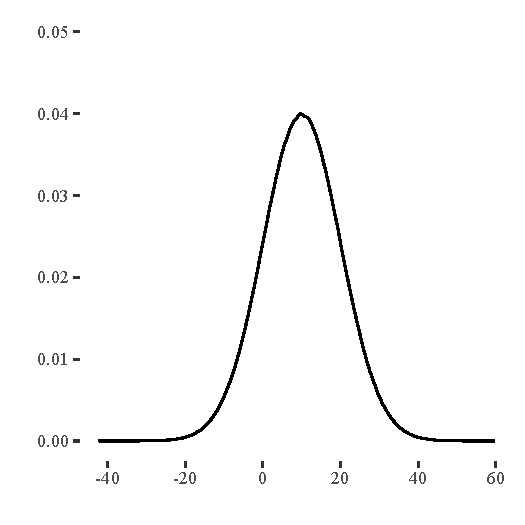
\includegraphics{AdditivityOfVariance_files/figure-latex/unnamed-chunk-8-1} 

}

\caption[$N(\mu_d, \sigma^2_d)$の分布]{$N(\mu_d, \sigma^2_d)$の分布}\label{fig:unnamed-chunk-8}
\end{marginfigure}

\begin{marginfigure}

{\centering 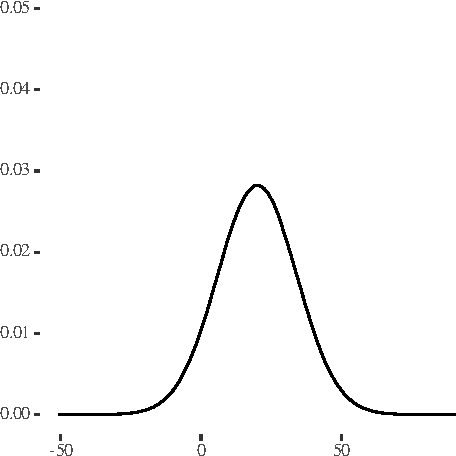
\includegraphics{AdditivityOfVariance_files/figure-latex/unnamed-chunk-9-1} 

}

\caption[$N(\mu_e, \sigma^2_e)$の分布]{$N(\mu_e, \sigma^2_e)$の分布}\label{fig:unnamed-chunk-9}
\end{marginfigure}

\newpage

\hypertarget{ux540cux4e00ux306eux6b63ux898fux5206ux5e03ux304bux3089ux53d6ux308aux51faux3057ux305fux5024ux3092ux5e73ux5747ux3057ux305fux5834ux5408}{%
\subsection{\texorpdfstring{\textbf{同一の正規分布から取り出した値を平均した場合}}{同一の正規分布から取り出した値を平均した場合}}\label{ux540cux4e00ux306eux6b63ux898fux5206ux5e03ux304bux3089ux53d6ux308aux51faux3057ux305fux5024ux3092ux5e73ux5747ux3057ux305fux5834ux5408}}

 同一の正規分布\(N(\mu_d, \sigma^2_d)\)から取り出した二つの値の\textbf{平均値の分布}を考えてみます。「二つの値の平均値の平均値」とは、正規分布\(N(\mu_d, \sigma^2_d)\)から、ランダムサンプリングで二つの値を取り出して、その平均値を取るということです。取り出した値は元の正規分布へ戻し、同様の操作を繰り返します。

\begin{Shaded}
\begin{Highlighting}[numbers=left,,]
\NormalTok{f }\OtherTok{\textless{}{-}} \FunctionTok{c}\NormalTok{((}\FunctionTok{sample}\NormalTok{(d, n, }\AttributeTok{replace =} \ConstantTok{TRUE}\NormalTok{) }\SpecialCharTok{+} \FunctionTok{sample}\NormalTok{(d, n, }\AttributeTok{replace =} \ConstantTok{TRUE}\NormalTok{)) }\SpecialCharTok{/} \DecValTok{2}\NormalTok{)}
\FunctionTok{head}\NormalTok{(f, }\DecValTok{20}\NormalTok{)}
\end{Highlighting}
\end{Shaded}

\begin{verbatim}
##  [1]  8.656109  6.365271 10.716425  1.298762  9.633547  9.873571  4.596933
##  [8] 11.911069 15.384756 12.053533 11.393067  1.115477 12.317064 10.701997
## [15] 15.624726 19.306380  8.377597  3.342314  6.966565 -2.440361
\end{verbatim}

この正規分布正規分布\(N(\mu_f, \sigma^2_f)\)は、二つの値の平均値、つまり二つの値を半分に割った値ですので正規分布\(N(2\mu_d, 2\sigma^2_d)\)のすべての値を半分にした正規分布になると予想できます。

\[\mbox{「二つの標本の平均値」の平均値} = \frac{2\mu_d}{2} = \mu_d\]

\[\mbox{「二つの標本の平均値」の標準偏差} = \frac{\sqrt{2}\sigma_d}{2} = \frac{\sigma_d}{\sqrt{2}}\]

\[\mbox{「二つの標本の平均値」の分散} = (\frac{\sigma_d}{\sqrt{2}})^2 = \frac{\sigma^2_d}{2}\]

\begin{marginfigure}

{\centering 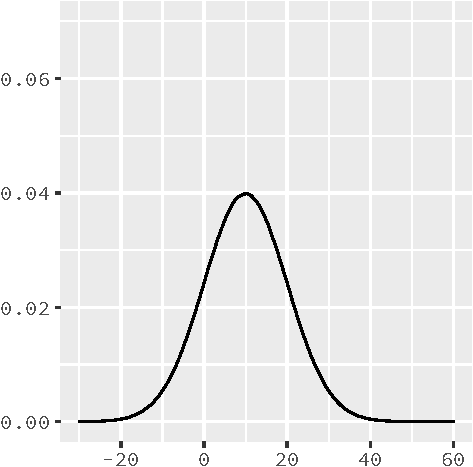
\includegraphics{AdditivityOfVariance_files/figure-latex/unnamed-chunk-11-1} 

}

\caption[$N(\mu_d, \sigma^2_d)$の分布]{$N(\mu_d, \sigma^2_d)$の分布}\label{fig:unnamed-chunk-11}
\end{marginfigure}

\begin{marginfigure}

{\centering 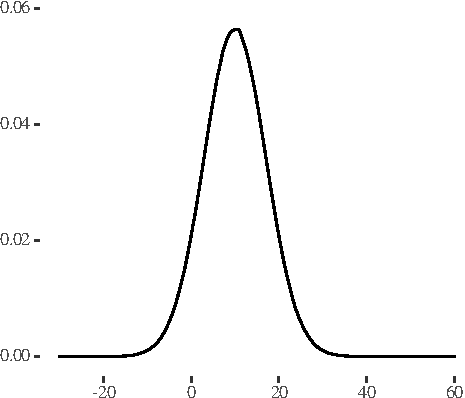
\includegraphics{AdditivityOfVariance_files/figure-latex/unnamed-chunk-12-1} 

}

\caption[$N(\mu_f, \sigma^2_f)$の分布]{$N(\mu_f, \sigma^2_f)$の分布}\label{fig:unnamed-chunk-12}
\end{marginfigure}

\begin{longtable}[]{@{}lcccl@{}}
\caption{各分布の要約統計量}\tabularnewline
\toprule
正規分布 & 平均 & 分散 & 標準偏差 & 備考 \\
\midrule
\endfirsthead
\toprule
正規分布 & 平均 & 分散 & 標準偏差 & 備考 \\
\midrule
\endhead
\(N(\mu_d, \sigma^2_d)\) & 9.997214 & 100.010064 & 10.0005032 &
元の分布 \\
\(N(\mu_d, \frac{\sigma^2_d}{2})\) & 9.997214 & 50.005032 & 7.0714236 &
分散の加法性 \\
\(N(\mu_f, \sigma^2_f)\) & 9.9943811 & 50.0335932 & 7.0734428 &
実際の分布 \\
\bottomrule
\end{longtable}

このように元の分布よりも鋭い分布になっていることがわかります。

\newpage

\hypertarget{ux4e09ux3064ux5024ux306eux5e73ux5747ux5024ux306eux5834ux5408}{%
\subsection{\texorpdfstring{\textbf{三つ値の平均値の場合}}{三つ値の平均値の場合}}\label{ux4e09ux3064ux5024ux306eux5e73ux5747ux5024ux306eux5834ux5408}}

 次に同一の正規分布\(N(\mu_d, \sigma^2_d)\)から取り出した三つの値の\textbf{平均値の分布}を考えてみます。
 

\begin{Shaded}
\begin{Highlighting}[numbers=left,,]
\NormalTok{g }\OtherTok{\textless{}{-}} \FunctionTok{c}\NormalTok{((}\FunctionTok{sample}\NormalTok{(d, n, }\AttributeTok{replace =} \ConstantTok{TRUE}\NormalTok{) }\SpecialCharTok{+} \FunctionTok{sample}\NormalTok{(d, n, }\AttributeTok{replace =} \ConstantTok{TRUE}\NormalTok{) }
        \SpecialCharTok{+} \FunctionTok{sample}\NormalTok{(d, n, }\AttributeTok{replace =} \ConstantTok{TRUE}\NormalTok{)) }\SpecialCharTok{/} \DecValTok{3}\NormalTok{)}
\FunctionTok{head}\NormalTok{(g, }\DecValTok{20}\NormalTok{)}
\end{Highlighting}
\end{Shaded}

\begin{verbatim}
##  [1]  9.9478545 26.1820143  6.5311987 17.3877299  6.2840528  9.3267385
##  [7] 10.2109100 18.8806762 16.1432096 10.6349812 22.8358974  0.1243132
## [13] 13.5626614  1.2668669 15.5944764 14.2404416 16.5512347 12.2533591
## [19]  6.4501340  6.1338214
\end{verbatim}

\begin{longtable}[]{@{}lcccl@{}}
\caption{各分布の要約統計量}\tabularnewline
\toprule
正規分布 & 平均 & 分散 & 標準偏差 & 備考 \\
\midrule
\endfirsthead
\toprule
正規分布 & 平均 & 分散 & 標準偏差 & 備考 \\
\midrule
\endhead
\(N(\mu_d, \sigma^2_d)\) & 9.997214 & 100.010064 & 10.0005032 &
元の分布 \\
\(N(\mu_g, \sigma^2_g)\) & 9.9936947 & 33.3155596 & 5.7719632 &
実際の分布 \\
比率 & 0.999648 & 0.3331221 & 0.5771673 & 元の分布に対する比率 \\
\bottomrule
\end{longtable}

標準偏差の比率(0.5771673)は、\(\frac{1}{\sqrt{3}} = 0.5773503\)とほぼ等しいことが分かります。これより

\[N(\mu_g, \sigma^2_g) = N(\mu_d, \frac{\sigma^2_d}{3})\]

となることがわかります。

\begin{marginfigure}

{\centering 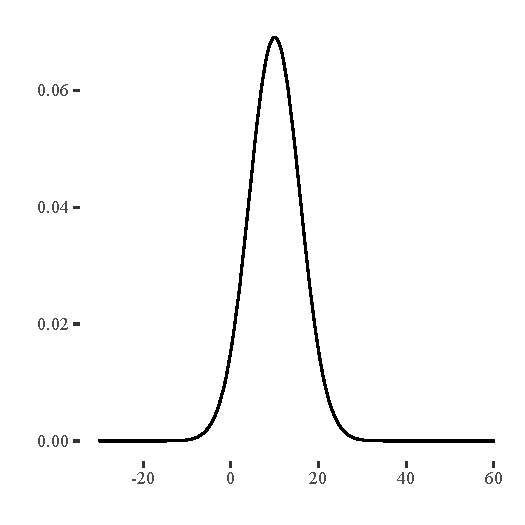
\includegraphics{AdditivityOfVariance_files/figure-latex/unnamed-chunk-14-1} 

}

\caption[$N(\mu_g, \sigma^2_g)$の分布]{$N(\mu_g, \sigma^2_g)$の分布}\label{fig:unnamed-chunk-14}
\end{marginfigure}

 

\hypertarget{ux4e00ux822cux5316ux3059ux308bux3068}{%
\subsection{\texorpdfstring{\textbf{一般化すると}}{一般化すると}}\label{ux4e00ux822cux5316ux3059ux308bux3068}}

 同一正規分布\(N(\mu, \sigma^2)\)から取り出した\(n\)個の値の\textbf{平均値の分布}\(N(\mu_, \sigma^2_n)\)は

\[N(\mu_n, \sigma^2_n) = N(\mu, \frac{\sigma^2}{n})\]

であり、平均は変わらず標準偏差が\(\frac{\sigma}{\sqrt{n}}\)となります。

\newpage

\hypertarget{ux304aux307eux3051ux5c0fux5ba4ux5148ux751fux306eux30a2ux30c9ux30d0ux30a4ux30b9ux304bux3089}{%
\section{\texorpdfstring{\textbf{おまけ}(小室先生のアドバイスから)}{おまけ(小室先生のアドバイスから)}}\label{ux304aux307eux3051ux5c0fux5ba4ux5148ux751fux306eux30a2ux30c9ux30d0ux30a4ux30b9ux304bux3089}}

 分散の加法性が成り立つには「データが独立」であるという前提条件があります。データが独立ということはデータ間の相関はないはずなので、乱数生成した二つのデータが本当に独立(無相関)なのかを確認します。

\begin{Shaded}
\begin{Highlighting}[numbers=left,,]
\NormalTok{f }\OtherTok{\textless{}{-}} \ControlFlowTok{function}\NormalTok{(}\AttributeTok{n =} \DecValTok{5000000}\NormalTok{) \{}
  \CommentTok{\# 乱数生成したデータ}
\NormalTok{  x }\OtherTok{\textless{}{-}} \FunctionTok{rnorm}\NormalTok{(}\AttributeTok{n =}\NormalTok{ n, }\AttributeTok{mean =} \DecValTok{10}\NormalTok{, }\AttributeTok{sd =} \DecValTok{10}\NormalTok{)}
\NormalTok{  y }\OtherTok{\textless{}{-}} \FunctionTok{rnorm}\NormalTok{(}\AttributeTok{n =}\NormalTok{ n, }\AttributeTok{mean =} \DecValTok{30}\NormalTok{, }\AttributeTok{sd =} \DecValTok{10}\NormalTok{)}
  \CommentTok{\# 乱数生成したデータ間の無相関の検定結果と要約統計量を結合}
  \FunctionTok{cor.test}\NormalTok{(x, y) }\SpecialCharTok{\%\textgreater{}\%}\NormalTok{ broom}\SpecialCharTok{::}\FunctionTok{tidy}\NormalTok{()}
\NormalTok{\}}
\end{Highlighting}
\end{Shaded}

上記の関数を繰り返し実行し結果を表示します。

\begin{Shaded}
\begin{Highlighting}[numbers=left,,]
\NormalTok{df }\OtherTok{\textless{}{-}} \FunctionTok{data.frame}\NormalTok{()}
\ControlFlowTok{for}\NormalTok{ (i }\ControlFlowTok{in} \FunctionTok{c}\NormalTok{(}\DecValTok{1}\SpecialCharTok{:}\DecValTok{100}\NormalTok{)) \{}
\NormalTok{  df }\OtherTok{\textless{}{-}}\NormalTok{ dplyr}\SpecialCharTok{::}\FunctionTok{bind\_rows}\NormalTok{(df, }\FunctionTok{f}\NormalTok{())}
\NormalTok{\}}

\NormalTok{df }\SpecialCharTok{\%\textgreater{}\%} 
\NormalTok{  dplyr}\SpecialCharTok{::}\FunctionTok{select}\NormalTok{(conf.low, }\AttributeTok{corr =}\NormalTok{ estimate, conf.high,}
\NormalTok{                p.value, }\AttributeTok{t.value =}\NormalTok{ statistic) }\SpecialCharTok{\%\textgreater{}\%} 
\NormalTok{  knitr}\SpecialCharTok{::}\FunctionTok{kable}\NormalTok{()}
\end{Highlighting}
\end{Shaded}

\begin{longtable}[]{@{}rrrrr@{}}
\toprule
conf.low & corr & conf.high & p.value & t.value \\
\midrule
\endhead
-0.0011882 & -0.0003116 & 0.0005649 & 0.4858912 & -0.6968587 \\
-0.0008757 & 0.0000008 & 0.0008773 & 0.9985939 & 0.0017623 \\
0.0003328 & 0.0012093 & 0.0020859 & 0.0068474 & 2.7041769 \\
-0.0002786 & 0.0005980 & 0.0014745 & 0.1811938 & 1.3370885 \\
-0.0012694 & -0.0003929 & 0.0004836 & 0.3796348 & -0.8785695 \\
-0.0010992 & -0.0002227 & 0.0006539 & 0.6185658 & -0.4978841 \\
-0.0013626 & -0.0004861 & 0.0003904 & 0.2770835 & -1.0868945 \\
-0.0006519 & 0.0002246 & 0.0011011 & 0.6155023 & 0.5022349 \\
-0.0009590 & -0.0000824 & 0.0007941 & 0.8537570 & -0.1843269 \\
-0.0005473 & 0.0003292 & 0.0012058 & 0.4616138 & 0.7361921 \\
-0.0010740 & -0.0001975 & 0.0006790 & 0.6587773 & -0.4416020 \\
-0.0001847 & 0.0006919 & 0.0015684 & 0.1218492 & 1.5470584 \\
-0.0001648 & 0.0007117 & 0.0015883 & 0.1114939 & 1.5915146 \\
-0.0007494 & 0.0001271 & 0.0010037 & 0.7761773 & 0.2843042 \\
-0.0000368 & 0.0008397 & 0.0017163 & 0.0604235 & 1.8776907 \\
-0.0005893 & 0.0002872 & 0.0011638 & 0.5206762 & 0.6423035 \\
-0.0006477 & 0.0002288 & 0.0011053 & 0.6088898 & 0.5116588 \\
-0.0007600 & 0.0001165 & 0.0009931 & 0.7944223 & 0.2605724 \\
-0.0001447 & 0.0007318 & 0.0016083 & 0.1017691 & 1.6363373 \\
-0.0014600 & -0.0005835 & 0.0002930 & 0.1919786 & -1.3047484 \\
-0.0005668 & 0.0003097 & 0.0011862 & 0.4885832 & 0.6925641 \\
-0.0010605 & -0.0001840 & 0.0006926 & 0.6808148 & -0.4113515 \\
-0.0014780 & -0.0006015 & 0.0002750 & 0.1786355 & -1.3449685 \\
-0.0003396 & 0.0005369 & 0.0014134 & 0.2299509 & 1.2004855 \\
-0.0011404 & -0.0002639 & 0.0006126 & 0.5551034 & -0.5901302 \\
-0.0008312 & 0.0000453 & 0.0009218 & 0.9193351 & 0.1012713 \\
-0.0001783 & 0.0006982 & 0.0015748 & 0.1184560 & 1.5612873 \\
0.0001928 & 0.0010693 & 0.0019458 & 0.0167996 & 2.3910650 \\
0.0000146 & 0.0008911 & 0.0017677 & 0.0462998 & 1.9926499 \\
-0.0013363 & -0.0004598 & 0.0004168 & 0.3039304 & -1.0280414 \\
-0.0010745 & -0.0001980 & 0.0006786 & 0.6580194 & -0.4426493 \\
-0.0017439 & -0.0008674 & 0.0000091 & 0.0524320 & -1.9395706 \\
-0.0005955 & 0.0002810 & 0.0011575 & 0.5298036 & 0.6283059 \\
-0.0009438 & -0.0000673 & 0.0008092 & 0.8803897 & -0.1504753 \\
-0.0010493 & -0.0001728 & 0.0007037 & 0.6992400 & -0.3863467 \\
-0.0005755 & 0.0003010 & 0.0011776 & 0.5008516 & 0.6731504 \\
-0.0012308 & -0.0003543 & 0.0005222 & 0.4282529 & -0.7921850 \\
-0.0013755 & -0.0004990 & 0.0003776 & 0.2645350 & -1.1157366 \\
-0.0009539 & -0.0000774 & 0.0007991 & 0.8625650 & -0.1731100 \\
-0.0001387 & 0.0007378 & 0.0016143 & 0.0989857 & 1.6497912 \\
-0.0006698 & 0.0002067 & 0.0010832 & 0.6439195 & 0.4622258 \\
-0.0007727 & 0.0001038 & 0.0009804 & 0.8164072 & 0.2321684 \\
-0.0008308 & 0.0000457 & 0.0009223 & 0.9185480 & 0.1022629 \\
-0.0014893 & -0.0006128 & 0.0002637 & 0.1705959 & -1.3702919 \\
-0.0003941 & 0.0004824 & 0.0013590 & 0.2807000 & 1.0787482 \\
-0.0004715 & 0.0004051 & 0.0012816 & 0.3650825 & 0.9057230 \\
-0.0007799 & 0.0000966 & 0.0009731 & 0.8290072 & 0.2159751 \\
-0.0011987 & -0.0003222 & 0.0005544 & 0.4713009 & -0.7203640 \\
-0.0007291 & 0.0001474 & 0.0010240 & 0.7416470 & 0.3296731 \\
-0.0009907 & -0.0001142 & 0.0007623 & 0.7984612 & -0.2553391 \\
-0.0005462 & 0.0003303 & 0.0012068 & 0.4601888 & 0.7385361 \\
-0.0005592 & 0.0003174 & 0.0011939 & 0.4779298 & 0.7096362 \\
-0.0000971 & 0.0007795 & 0.0016560 & 0.0813498 & 1.7429077 \\
-0.0004972 & 0.0003794 & 0.0012559 & 0.3962801 & 0.8482836 \\
-0.0007113 & 0.0001652 & 0.0010418 & 0.7117756 & 0.3694725 \\
-0.0007202 & 0.0001564 & 0.0010329 & 0.7265946 & 0.3496591 \\
-0.0006672 & 0.0002093 & 0.0010859 & 0.6397313 & 0.4680745 \\
-0.0007866 & 0.0000899 & 0.0009665 & 0.8405969 & 0.2011301 \\
-0.0008804 & -0.0000038 & 0.0008727 & 0.9931615 & -0.0085709 \\
-0.0003494 & 0.0005272 & 0.0014037 & 0.2384985 & 1.1787482 \\
-0.0005889 & 0.0002876 & 0.0011641 & 0.5201552 & 0.6431063 \\
-0.0007369 & 0.0001396 & 0.0010161 & 0.7549505 & 0.3121185 \\
-0.0003494 & 0.0005271 & 0.0014037 & 0.2385108 & 1.1787172 \\
0.0001365 & 0.0010130 & 0.0018896 & 0.0234993 & 2.2652181 \\
-0.0005242 & 0.0003524 & 0.0012289 & 0.4307485 & 0.7879114 \\
-0.0004443 & 0.0004323 & 0.0013088 & 0.3337542 & 0.9665798 \\
-0.0014243 & -0.0005478 & 0.0003288 & 0.2206407 & -1.2248265 \\
0.0000009 & 0.0008775 & 0.0017540 & 0.0497549 & 1.9620660 \\
-0.0015014 & -0.0006249 & 0.0002516 & 0.1623039 & -1.3973649 \\
-0.0008036 & 0.0000729 & 0.0009495 & 0.8704464 & 0.1630915 \\
-0.0013561 & -0.0004795 & 0.0003970 & 0.2836007 & -1.0722659 \\
-0.0003792 & 0.0004974 & 0.0013739 & 0.2660874 & 1.1121183 \\
-0.0019344 & -0.0010579 & -0.0001814 & 0.0180024 & -2.3655699 \\
-0.0009997 & -0.0001232 & 0.0007533 & 0.7829672 & -0.2754544 \\
-0.0007300 & 0.0001465 & 0.0010231 & 0.7431586 & 0.3276734 \\
-0.0005485 & 0.0003280 & 0.0012045 & 0.4632905 & 0.7334393 \\
-0.0008352 & 0.0000413 & 0.0009179 & 0.9263420 & 0.0924481 \\
-0.0011643 & -0.0002878 & 0.0005888 & 0.5199296 & -0.6434540 \\
-0.0009044 & -0.0000279 & 0.0008486 & 0.9502210 & -0.0624293 \\
-0.0012892 & -0.0004127 & 0.0004638 & 0.3560962 & -0.9228293 \\
-0.0008035 & 0.0000731 & 0.0009496 & 0.8702434 & 0.1633493 \\
-0.0011117 & -0.0002351 & 0.0006414 & 0.5990309 & -0.5257946 \\
-0.0003306 & 0.0005459 & 0.0014224 & 0.2222061 & 1.2206831 \\
-0.0003539 & 0.0005226 & 0.0013991 & 0.2425647 & 1.1686005 \\
-0.0002734 & 0.0006031 & 0.0014796 & 0.1774627 & 1.3486087 \\
-0.0021564 & -0.0012798 & -0.0004033 & 0.0042123 & -2.8618098 \\
-0.0013014 & -0.0004249 & 0.0004517 & 0.3421073 & -0.9500099 \\
-0.0003791 & 0.0004974 & 0.0013739 & 0.2660645 & 1.1121714 \\
-0.0013231 & -0.0004466 & 0.0004299 & 0.3179732 & -0.9986317 \\
-0.0007080 & 0.0001685 & 0.0010451 & 0.7062847 & 0.3768505 \\
-0.0010910 & -0.0002144 & 0.0006621 & 0.6315721 & -0.4795153 \\
-0.0005022 & 0.0003743 & 0.0012508 & 0.4026436 & 0.8369093 \\
-0.0008326 & 0.0000439 & 0.0009205 & 0.9217432 & 0.0982381 \\
-0.0007503 & 0.0001263 & 0.0010028 & 0.7776817 & 0.2823415 \\
-0.0005507 & 0.0003258 & 0.0012024 & 0.4662466 & 0.7285997 \\
-0.0014904 & -0.0006139 & 0.0002626 & 0.1698304 & -1.3727492 \\
0.0001231 & 0.0009997 & 0.0018762 & 0.0253961 & 2.2353239 \\
-0.0007870 & 0.0000895 & 0.0009660 & 0.8414089 & 0.2000917 \\
-0.0011532 & -0.0002767 & 0.0005998 & 0.5360922 & -0.6187331 \\
-0.0011201 & -0.0002436 & 0.0006329 & 0.5859491 & -0.5447157 \\
\bottomrule
\end{longtable}

得られた結果の内、有意水準\(\alpha = 0.05\)で帰無仮説が棄却(\(p < \alpha\))されるケースを抽出します。

\begin{Shaded}
\begin{Highlighting}[numbers=left,,]
\NormalTok{df }\SpecialCharTok{\%\textgreater{}\%} 
\NormalTok{  dplyr}\SpecialCharTok{::}\FunctionTok{select}\NormalTok{(conf.low, }\AttributeTok{corr =}\NormalTok{ estimate, conf.high,}
\NormalTok{                p.value, }\AttributeTok{t.value =}\NormalTok{ statistic) }\SpecialCharTok{\%\textgreater{}\%} 
\NormalTok{  dplyr}\SpecialCharTok{::}\FunctionTok{filter}\NormalTok{(p.value }\SpecialCharTok{\textless{}} \FloatTok{0.05}\NormalTok{) }\SpecialCharTok{\%\textgreater{}\%} 
\NormalTok{  knitr}\SpecialCharTok{::}\FunctionTok{kable}\NormalTok{()}
\end{Highlighting}
\end{Shaded}

\begin{longtable}[]{@{}rrrrr@{}}
\toprule
conf.low & corr & conf.high & p.value & t.value \\
\midrule
\endhead
0.0003328 & 0.0012093 & 0.0020859 & 0.0068474 & 2.704177 \\
0.0001928 & 0.0010693 & 0.0019458 & 0.0167996 & 2.391065 \\
0.0000146 & 0.0008911 & 0.0017677 & 0.0462998 & 1.992650 \\
0.0001365 & 0.0010130 & 0.0018896 & 0.0234993 & 2.265218 \\
0.0000009 & 0.0008775 & 0.0017540 & 0.0497549 & 1.962066 \\
-0.0019344 & -0.0010579 & -0.0001814 & 0.0180024 & -2.365570 \\
-0.0021564 & -0.0012798 & -0.0004033 & 0.0042123 & -2.861810 \\
0.0001231 & 0.0009997 & 0.0018762 & 0.0253961 & 2.235324 \\
\bottomrule
\end{longtable}

 

乱数生成した二つのデータからそれぞれランダムサンプリングを行った場合(観測で得られたデータに相当)についても同様に確認してみます。

\begin{Shaded}
\begin{Highlighting}[numbers=left,,]
\NormalTok{fs }\OtherTok{\textless{}{-}} \ControlFlowTok{function}\NormalTok{(}\AttributeTok{n =} \DecValTok{5000000}\NormalTok{) \{}
  \CommentTok{\# 乱数生成したデータをランダムサンプリングする}
\NormalTok{  x }\OtherTok{\textless{}{-}} \FunctionTok{rnorm}\NormalTok{(}\AttributeTok{n =}\NormalTok{ n, }\AttributeTok{mean =} \DecValTok{10}\NormalTok{, }\AttributeTok{sd =} \DecValTok{10}\NormalTok{) }\SpecialCharTok{\%\textgreater{}\%} \FunctionTok{sample}\NormalTok{(n, }\AttributeTok{replace =} \ConstantTok{TRUE}\NormalTok{)}
\NormalTok{  y }\OtherTok{\textless{}{-}} \FunctionTok{rnorm}\NormalTok{(}\AttributeTok{n =}\NormalTok{ n, }\AttributeTok{mean =} \DecValTok{30}\NormalTok{, }\AttributeTok{sd =} \DecValTok{10}\NormalTok{) }\SpecialCharTok{\%\textgreater{}\%} \FunctionTok{sample}\NormalTok{(n, }\AttributeTok{replace =} \ConstantTok{TRUE}\NormalTok{)}
  \CommentTok{\# ランダムサンプリングしたデータ間の無相関の検定結果と要約統計量を結合}
  \FunctionTok{cor.test}\NormalTok{(x, y) }\SpecialCharTok{\%\textgreater{}\%}\NormalTok{ broom}\SpecialCharTok{::}\FunctionTok{tidy}\NormalTok{()}
\NormalTok{\}}

\NormalTok{df }\OtherTok{\textless{}{-}} \FunctionTok{data.frame}\NormalTok{()}
\ControlFlowTok{for}\NormalTok{ (i }\ControlFlowTok{in} \FunctionTok{c}\NormalTok{(}\DecValTok{1}\SpecialCharTok{:}\DecValTok{100}\NormalTok{)) \{}
\NormalTok{  df }\OtherTok{\textless{}{-}}\NormalTok{ dplyr}\SpecialCharTok{::}\FunctionTok{bind\_rows}\NormalTok{(df, }\FunctionTok{fs}\NormalTok{())}
\NormalTok{\}}

\NormalTok{df }\SpecialCharTok{\%\textgreater{}\%} 
\NormalTok{  dplyr}\SpecialCharTok{::}\FunctionTok{select}\NormalTok{(conf.low, }\AttributeTok{corr =}\NormalTok{ estimate, conf.high,}
\NormalTok{                p.value, }\AttributeTok{t.value =}\NormalTok{ statistic) }\SpecialCharTok{\%\textgreater{}\%} 
\NormalTok{  knitr}\SpecialCharTok{::}\FunctionTok{kable}\NormalTok{()}
\end{Highlighting}
\end{Shaded}

\begin{longtable}[]{@{}rrrrr@{}}
\toprule
conf.low & corr & conf.high & p.value & t.value \\
\midrule
\endhead
-0.0006881 & 0.0001884 & 0.0010650 & 0.6734794 & 0.4213776 \\
-0.0008852 & -0.0000087 & 0.0008678 & 0.9845254 & -0.0193957 \\
-0.0011018 & -0.0002253 & 0.0006512 & 0.6144368 & -0.5037504 \\
-0.0019009 & -0.0010244 & -0.0001479 & 0.0219859 & -2.2906127 \\
-0.0003452 & 0.0005313 & 0.0014078 & 0.2348103 & 1.1880589 \\
-0.0010522 & -0.0001756 & 0.0007009 & 0.6945015 & -0.3927536 \\
-0.0007706 & 0.0001059 & 0.0009824 & 0.8128574 & 0.2367415 \\
-0.0007872 & 0.0000894 & 0.0009659 & 0.8416394 & 0.1997970 \\
-0.0001844 & 0.0006922 & 0.0015687 & 0.1216896 & 1.5477207 \\
-0.0008810 & -0.0000045 & 0.0008720 & 0.9919644 & -0.0100713 \\
-0.0016718 & -0.0007953 & 0.0000812 & 0.0753375 & -1.7784044 \\
-0.0013875 & -0.0005109 & 0.0003656 & 0.2532454 & -1.1425022 \\
-0.0012608 & -0.0003843 & 0.0004922 & 0.3901354 & -0.8593720 \\
-0.0004965 & 0.0003800 & 0.0012565 & 0.3954676 & 0.8497437 \\
-0.0008389 & 0.0000377 & 0.0009142 & 0.9329058 & 0.0841895 \\
-0.0005163 & 0.0003602 & 0.0012367 & 0.4205979 & 0.8053844 \\
-0.0008453 & 0.0000312 & 0.0009077 & 0.9444213 & 0.0697140 \\
-0.0000942 & 0.0007823 & 0.0016588 & 0.0802381 & 1.7493064 \\
-0.0009866 & -0.0001101 & 0.0007665 & 0.8056113 & -0.2460917 \\
-0.0004837 & 0.0003928 & 0.0012693 & 0.3797351 & 0.8783845 \\
-0.0011649 & -0.0002884 & 0.0005881 & 0.5190026 & -0.6448837 \\
-0.0005201 & 0.0003564 & 0.0012330 & 0.4254437 & 0.7970127 \\
-0.0012974 & -0.0004209 & 0.0004556 & 0.3466508 & -0.9411057 \\
-0.0005361 & 0.0003405 & 0.0012170 & 0.4464842 & 0.7612895 \\
-0.0014711 & -0.0005946 & 0.0002819 & 0.1836679 & -1.3295460 \\
-0.0009434 & -0.0000669 & 0.0008096 & 0.8811036 & -0.1495704 \\
-0.0007856 & 0.0000909 & 0.0009675 & 0.8388496 & 0.2033652 \\
-0.0005564 & 0.0003201 & 0.0011967 & 0.4740812 & 0.7158545 \\
-0.0019995 & -0.0011230 & -0.0002465 & 0.0120358 & -2.5110938 \\
-0.0010786 & -0.0002021 & 0.0006744 & 0.6512922 & -0.4519678 \\
-0.0002719 & 0.0006046 & 0.0014812 & 0.1763678 & 1.3520236 \\
-0.0008162 & 0.0000603 & 0.0009368 & 0.8927821 & 0.1347847 \\
-0.0002388 & 0.0006377 & 0.0015142 & 0.1538971 & 1.4259007 \\
-0.0007376 & 0.0001389 & 0.0010154 & 0.7560860 & 0.3106247 \\
-0.0004382 & 0.0004384 & 0.0013149 & 0.3269947 & 0.9801853 \\
-0.0006832 & 0.0001934 & 0.0010699 & 0.6654662 & 0.4323787 \\
-0.0003629 & 0.0005136 & 0.0013901 & 0.2507916 & 1.1484290 \\
-0.0013567 & -0.0004802 & 0.0003963 & 0.2829216 & -1.0737795 \\
-0.0011486 & -0.0002720 & 0.0006045 & 0.5430040 & -0.6082767 \\
-0.0016034 & -0.0007269 & 0.0001496 & 0.1040655 & -1.6254561 \\
-0.0009287 & -0.0000522 & 0.0008244 & 0.9071539 & -0.1166293 \\
-0.0004581 & 0.0004184 & 0.0012950 & 0.3494430 & 0.9356704 \\
-0.0015536 & -0.0006771 & 0.0001994 & 0.1300037 & -1.5140877 \\
-0.0006800 & 0.0001965 & 0.0010730 & 0.6603772 & 0.4393924 \\
-0.0008239 & 0.0000526 & 0.0009291 & 0.9063849 & 0.1175996 \\
-0.0009496 & -0.0000731 & 0.0008035 & 0.8702457 & -0.1633464 \\
-0.0010279 & -0.0001513 & 0.0007252 & 0.7350542 & -0.3384101 \\
-0.0007701 & 0.0001064 & 0.0009829 & 0.8119254 & 0.2379429 \\
-0.0022496 & -0.0013730 & -0.0004965 & 0.0021392 & -3.0701932 \\
-0.0008833 & -0.0000067 & 0.0008698 & 0.9879645 & -0.0150848 \\
-0.0008889 & -0.0000124 & 0.0008642 & 0.9779446 & -0.0276459 \\
-0.0021426 & -0.0012661 & -0.0003896 & 0.0046397 & -2.8310437 \\
-0.0006137 & 0.0002628 & 0.0011394 & 0.5567189 & 0.5877221 \\
-0.0011816 & -0.0003050 & 0.0005715 & 0.4951737 & -0.6821032 \\
-0.0008802 & -0.0000037 & 0.0008729 & 0.9934879 & -0.0081618 \\
-0.0003607 & 0.0005158 & 0.0013923 & 0.2487637 & 1.1533576 \\
-0.0002880 & 0.0005885 & 0.0014650 & 0.1881887 & 1.3159565 \\
-0.0011265 & -0.0002500 & 0.0006265 & 0.5761682 & -0.5589905 \\
-0.0009220 & -0.0000455 & 0.0008311 & 0.9190145 & -0.1016752 \\
-0.0016460 & -0.0007695 & 0.0001070 & 0.0853181 & -1.7206298 \\
-0.0003015 & 0.0005750 & 0.0014515 & 0.1985359 & 1.2857342 \\
-0.0006020 & 0.0002745 & 0.0011510 & 0.5393106 & 0.6138559 \\
-0.0014461 & -0.0005696 & 0.0003069 & 0.2027770 & -1.2736798 \\
-0.0008434 & 0.0000332 & 0.0009097 & 0.9408736 & 0.0741719 \\
-0.0013021 & -0.0004256 & 0.0004509 & 0.3412694 & -0.9516603 \\
-0.0006416 & 0.0002349 & 0.0011114 & 0.5994008 & 0.5252625 \\
-0.0001120 & 0.0007645 & 0.0016410 & 0.0873740 & 1.7094158 \\
-0.0012900 & -0.0004134 & 0.0004631 & 0.3552270 & -0.9244982 \\
-0.0007274 & 0.0001492 & 0.0010257 & 0.7387347 & 0.3335294 \\
-0.0007182 & 0.0001583 & 0.0010349 & 0.7233149 & 0.3540320 \\
-0.0012996 & -0.0004231 & 0.0004534 & 0.3441301 & -0.9460363 \\
-0.0006959 & 0.0001806 & 0.0010571 & 0.6863622 & 0.4037967 \\
-0.0015430 & -0.0006664 & 0.0002101 & 0.1361706 & -1.4902041 \\
-0.0010184 & -0.0001418 & 0.0007347 & 0.7511258 & -0.3171553 \\
-0.0016168 & -0.0007402 & 0.0001363 & 0.0978818 & -1.6552108 \\
-0.0006226 & 0.0002539 & 0.0011305 & 0.5701399 & 0.5678455 \\
-0.0009117 & -0.0000352 & 0.0008413 & 0.9372678 & -0.0787043 \\
-0.0007960 & 0.0000805 & 0.0009570 & 0.8571456 & 0.1800089 \\
-0.0000100 & 0.0008666 & 0.0017431 & 0.0526580 & 1.9377152 \\
-0.0007868 & 0.0000897 & 0.0009662 & 0.8410252 & 0.2005823 \\
-0.0013187 & -0.0004422 & 0.0004344 & 0.3228150 & -0.9886898 \\
-0.0013869 & -0.0005104 & 0.0003661 & 0.2537401 & -1.1413120 \\
-0.0012656 & -0.0003891 & 0.0004875 & 0.3843132 & -0.8699767 \\
-0.0009346 & -0.0000581 & 0.0008184 & 0.8966633 & -0.1298776 \\
-0.0008433 & 0.0000332 & 0.0009098 & 0.9407651 & 0.0743082 \\
-0.0016399 & -0.0007633 & 0.0001132 & 0.0878486 & -1.7068574 \\
-0.0014134 & -0.0005368 & 0.0003397 & 0.2299764 & -1.2004197 \\
-0.0010562 & -0.0001797 & 0.0006969 & 0.6878664 & -0.4017523 \\
-0.0005646 & 0.0003120 & 0.0011885 & 0.4854569 & 0.6975529 \\
-0.0005607 & 0.0003158 & 0.0011923 & 0.4801120 & 0.7061224 \\
-0.0008916 & -0.0000151 & 0.0008614 & 0.9730435 & -0.0337914 \\
-0.0008238 & 0.0000527 & 0.0009293 & 0.9061179 & 0.1179367 \\
-0.0006973 & 0.0001792 & 0.0010557 & 0.6886471 & 0.4006918 \\
-0.0013219 & -0.0004453 & 0.0004312 & 0.3193402 & -0.9958149 \\
-0.0018141 & -0.0009376 & -0.0000610 & 0.0360441 & -2.0964297 \\
-0.0006996 & 0.0001769 & 0.0010534 & 0.6924604 & 0.3955184 \\
0.0002706 & 0.0011471 & 0.0020236 & 0.0103169 & 2.5650233 \\
-0.0011907 & -0.0003142 & 0.0005624 & 0.4823746 & -0.7024886 \\
-0.0010411 & -0.0001646 & 0.0007119 & 0.7128092 & -0.3680859 \\
-0.0003629 & 0.0005136 & 0.0013901 & 0.2507705 & 1.1484801 \\
\bottomrule
\end{longtable}

\begin{Shaded}
\begin{Highlighting}[numbers=left,,]
\NormalTok{df }\SpecialCharTok{\%\textgreater{}\%} 
\NormalTok{  dplyr}\SpecialCharTok{::}\FunctionTok{select}\NormalTok{(conf.low, }\AttributeTok{corr =}\NormalTok{ estimate, conf.high,}
\NormalTok{                p.value, }\AttributeTok{t.value =}\NormalTok{ statistic) }\SpecialCharTok{\%\textgreater{}\%} 
\NormalTok{  dplyr}\SpecialCharTok{::}\FunctionTok{filter}\NormalTok{(p.value }\SpecialCharTok{\textless{}} \FloatTok{0.05}\NormalTok{) }\SpecialCharTok{\%\textgreater{}\%} 
\NormalTok{  knitr}\SpecialCharTok{::}\FunctionTok{kable}\NormalTok{()}
\end{Highlighting}
\end{Shaded}

\begin{longtable}[]{@{}rrrrr@{}}
\toprule
conf.low & corr & conf.high & p.value & t.value \\
\midrule
\endhead
-0.0019009 & -0.0010244 & -0.0001479 & 0.0219859 & -2.290613 \\
-0.0019995 & -0.0011230 & -0.0002465 & 0.0120358 & -2.511094 \\
-0.0022496 & -0.0013730 & -0.0004965 & 0.0021392 & -3.070193 \\
-0.0021426 & -0.0012661 & -0.0003896 & 0.0046397 & -2.831044 \\
-0.0018141 & -0.0009376 & -0.0000610 & 0.0360441 & -2.096430 \\
0.0002706 & 0.0011471 & 0.0020236 & 0.0103169 & 2.565023 \\
\bottomrule
\end{longtable}

 

\hypertarget{ux307eux3068ux3081}{%
\subsection{まとめ}\label{ux307eux3068ux3081}}

 無相関の検定が成功するケース(\(95\%\)信頼区間に\(0\)が入らない)があるものの、その場合でも相関係数がゼロから大きく外れてはいない(極めてゼロに近い値になっている)ため、乱数生成した二つのデータ、ならびに、乱数生成した二つのデータからランダムサンプリングした二つのデータは、どちらも独立していると考えて差し支えないかと。

 

\hypertarget{cor.testux95a2ux6570ux306bux3064ux3044ux3066}{%
\subsection{\texorpdfstring{\texttt{cor.test()}関数について}{cor.test()関数について}}\label{cor.testux95a2ux6570ux306bux3064ux3044ux3066}}

 \texttt{cor.test()}関数は無相関の検定を行う関数です。対立仮説(\(H_1\))は下記の出力の通り「true
correlation is \textbf{not} equal to
0(相関係数はゼロではない)」ですので、帰無仮説(\(H_0\))は「相関係数はゼロである(相関はない)」となります。有意水準\(\alpha\)で検定が失敗すれば(帰無仮説が棄却されない、\(p \geqq \alpha\)である)帰無仮説が採択されますので相関係数はゼロ(データ間には相関がない)と考えられます。

\begin{verbatim}
## 
##  Pearson's product-moment correlation
## 
## data:  rnorm(n) and rnorm(n)
## t = 0.46682, df = 4999998, p-value = 0.6406
## alternative hypothesis: true correlation is not equal to 0
## 95 percent confidence interval:
##  -0.0006677559  0.0010852891
## sample estimates:
##          cor 
## 0.0002087668
\end{verbatim}

\newpage

\hypertarget{appendix}{%
\section{Appendix}\label{appendix}}

\hypertarget{about-handout-style}{%
\subsection{About handout style}\label{about-handout-style}}

The Tufte handout style is a style that Edward Tufte uses in his books
and handouts. Tufte's style is known for its extensive use of sidenotes,
tight integration of graphics with text, and well-set typography. This
style has been implemented in LaTeX and HTML/CSS\footnote{See Github
  repositories
  \href{https://github.com/tufte-latex/tufte-latex}{tufte-latex} and
  \href{https://github.com/edwardtufte/tufte-css}{tufte-css}},
respectively.

 

\bibliography{bib/references.bib}



\end{document}
